\documentclass[../../FisicaTeorica.tex]{subfiles}

%%%PACKAGES
\usepackage[usenames, dvipsnames, table]{xcolor}
\usepackage[utf8]{inputenc}
\usepackage[T1]{fontenc}
\usepackage{lmodern}
\usepackage{amsmath}
\usepackage{amsthm}
\usepackage{amsfonts}
\usepackage{comment}
\usepackage{wrapfig}
\usepackage{booktabs}
\usepackage{braket}
\usepackage{pgf,tikz}
\usepackage{mathrsfs}
\usetikzlibrary{arrows}
\usepackage{subfigure}
\usepackage{xspace}
\usepackage{gnuplottex}
\usepackage{epstopdf}
\usepackage{marginnote}
\usepackage{float}
\usetikzlibrary{tikzmark}
\usepackage{graphicx}
\usepackage{cancel}
\usepackage{bm}
\usepackage{mathtools}
\usepackage{hyperref}
\usepackage{ragged2e}
\usepackage[stable]{footmisc}
\usepackage{enumerate}
\usepackage{mathdots}
\usepackage[framemethod=tikz]{mdframed}
\PassOptionsToPackage{table}{xcolor}
\usepackage{soul}
\usepackage{enumerate}
\usepackage{mathdots}
\usepackage[framemethod=tikz]{mdframed} %Added 16/10
\usepackage[italian]{babel} %Added 16/10
\usepackage{amssymb} %Added
\usepackage{enumitem}
\usepackage{array}


%%BOOKTAB
\setlength{\aboverulesep}{0pt}
\setlength{\belowrulesep}{0pt}
\setlength{\extrarowheight}{.75ex}
\setlength\parindent{0pt} %Rimuove indentazione


%%GEOMETRIA
\usepackage[a4paper]{geometry}
 \newgeometry{inner=20mm,
            outer=49mm,% = marginparsep + marginparwidth 
                       %   + 5mm (between marginpar and page border)
            top=20mm,
            bottom=25mm,
            marginparsep=6mm,
            marginparwidth=30mm}
\makeatletter
\renewcommand{\@marginparreset}{%
  \reset@font\small
  \raggedright
  \slshape
  \@setminipage
}
\makeatother
 

%%COMANDI
\newcommand{\q}[1]{``#1''}
\newcommand{\lamb}[2]{\Lambda^{#1}_{\>{#2}}}
\newcommand{\norm}[1]{\left\lVert#1\right\rVert}
\newcommand{\hs}{\mathcal{H}}
\newcommand{\minus}{\scalebox{0.75}[1.0]{$-$}}
\newcommand{\hlc}[2]{%
  \colorbox{#1!50}{$\displaystyle#2$}}
\newcommand{\bb}[1]{\mathbb{#1}}
\newcommand{\op}[1]{\operatorname{#1}}
\renewcommand{\figurename}{Fig.}
\newcommand{\dom}[1]{D#1}
\newcommand{\avg}[1]{\left\langle{#1}\right\rangle}
\newcommand{\NN}{\mathbb N}
\newcommand{\RR}{\mathbb R}
\newcommand{\CC}{\mathbb C}
\newcommand{\mS}{\mathcal S}
\newcommand{\de}{d}
\newcommand{\abs}[1]{\left|#1\right|}

\newcommand{\lesson}[2]{\marginpar{(Lezione #1 del #2)}}
\DeclareRobustCommand{\MQ}{{\small\textsc{MQ}}\xspace}
\DeclareRobustCommand{\MC}{{\small\textsc{MC}}\xspace}
%Prima era \small\textsc{MQ}\xspace

%%TESTATINE
\usepackage{fancyhdr}
\pagestyle{fancy}
\fancyhead{} % clear all header fields
\renewcommand{\headrulewidth}{0pt} % no line in header area
\fancyfoot{} % clear all footer fields
%\fancyfoot[R]{A.A. 2018/19} % other info in "inner" position of footer line
\cfoot{\thepage}


%%AMBIENTI
\theoremstyle{plain}
\newtheorem{thm}{Teorema}[section]
\newtheorem{lem}{Lemma}[section]
\newtheorem{prop}{Proposizione}[section]
\newtheorem{axi}{Assioma}
\newtheorem{pst}{Postulato}

\theoremstyle{definition}
\newtheorem{dfn}{Definizione}

\theoremstyle{remark}
\newtheorem{oss}{Osservazione}
\newtheorem{es}{Esempio}
\newtheorem{ex}{Esercizio}

%Spiegazioni/verifiche
\newenvironment{expl}{\begin{mdframed}[hidealllines=true,backgroundcolor=green!20,innerleftmargin=3pt,innerrightmargin=3pt,leftmargin=-3pt,rightmargin=-3pt]}{\end{mdframed}} %Box di colore verde

\newenvironment{appr}{\begin{mdframed}[hidealllines=true,backgroundcolor=blue!10,innerleftmargin=3pt,innerrightmargin=3pt,leftmargin=-3pt,rightmargin=-3pt]}{\end{mdframed}} %Approfondimenti matematici (box di colore blu)

%%Domande di Marchetti
\newtheorem{question}{Domanda}


%%OPERATORI
\DeclareMathOperator{\sech}{sech}
\DeclareMathOperator{\csch}{csch}
\DeclareMathOperator{\arcsec}{arcsec}
\DeclareMathOperator{\arccot}{arcCot}
\DeclareMathOperator{\arccsc}{arcCsc}
\DeclareMathOperator{\arccosh}{arcCosh}
\DeclareMathOperator{\arcsinh}{arcsinh}
\DeclareMathOperator{\arctanh}{arctanh}
\DeclareMathOperator{\arcsech}{arcsech}
\DeclareMathOperator{\arccsch}{arcCsch}
\DeclareMathOperator{\arccoth}{arcCoth} 




\begin{document}

\subsection{Autoaggiuntezza in dimensione $\infty$: famiglie spettrali}
Potremmo essere tentati di estendere questa\marginpar{Decomposizione spettrale in $\op{dim}\hs =\infty$: problemi iniziali} strategia per costruire una funzione di un'osservabile $O$ ($f(O)$) anche nel caso $\op{dim}\hs = \infty$, per esempio in $\hs = L^2(\bb{R}, dx)$.\\
Tuttavia, ciò porta subito a dei problemi.\\
Per esempio, sia $X$ l'operatore autoaggiunto ($X=X^\dag$) con dominio $D(X) = \{\psi \in L^2(\bb{R}, dx)\>|\>x\psi \in L^2(\bb{R})\}$ che agisce su $\psi$ come $X\psi = x\psi$.\\
Allora l'equazione agli autovalori diviene:
\[
X\psi_\lambda (x) = \lambda \psi_\lambda (x)
\]
Applicando la definizione di $X$:
\[
X\psi_\lambda(x) = x\psi_\lambda(x) \Rightarrow (x-\lambda)\psi_\lambda (x) = 0
\]
Scartiamo la soluzione banale $\psi_\lambda(x) \equiv 0$ che non è fisica\footnote{La posizione di una particella non può essere \q{da nessuna parte}!}, ma allora l'equazione di sopra deve valere solo per $x = \lambda$.\\
Tuttavia $\{x = \lambda \}$ ha misura di Lebesgue nulla: in altre parole stiamo cercando una soluzione (non nulla) che sia $0$ per tutte le $x$ tranne $\lambda$ (ossia tranne un insieme Lebesgue-trascurabile). Ma tale funzione, in $L^2$, è quella nulla, che abbiamo appena scartato!\\
Siamo costretti ad affermare perciò che $X$ non possiede autovettori - e con ciò termina il primo tentativo di generalizzare la decomposizione spettrale al caso infinito-dimensionale: come possiamo trovare una base ON di autovettori se di autovettori non ce ne sono?\\

Proviamo a tornare al caso $\op{dim}\hs < \infty$ e studiare una strategia alternativa che possa essere generalizzata.\\
Poco fa, per dimostrare che gli autovalori \q{matematici} (di un operatore) sono tutti e soli quelli \q{fisici} (dell'osservabile rappresentato) nel caso finito-dimensionale avevamo fatto uso di un argomento probabilistico (le probabilità $p_n$ associate agli autovalori $\lambda_n$ \textit{esauriscono} tutte le possibilità). Potremmo perciò cercare di partire da qui, riesaminando la struttura probabilistica nel caso finito-dimensionale - essenzialmente declinando quanto detto nei paragrafi di descrizione di un sistema fisico %Inserire ref alla parte di probabilità dopo teoria della misura
alla luce di quanto appena visto sulle proprietà degli operatori e sulla decomposizione spettrale.\\
Partiamo\marginpar{Struttura probabilistica per operatori in \MQ} dallo scrivere l'equivalente di (\ref{eqn:POdef})\footnote{$P^O(\lambda) = H(\lambda-O)$} per un operatore, tramite la decomposizione spettrale: %[REF]
\begin{equation} 
P^A\left(\lambda\right)=\sum_{n}{H\left(\lambda-\lambda_n\right)P_n}\equiv H(\lambda \mathbb{I} - A) 
\label{eqn:PA}
\end{equation}
(che si intende valida per ogni stato $\psi$. Nota: con $P^A(\lambda)$ indichiamo un operatore che dipende da $\lambda$, non una funzione reale a valori reali!)\\
Ma allora da (\ref{eqn:Omedio})\footnote{$\langle O \rangle_\Sigma = \int_\bb{R} \lambda\, d\langle H(\lambda-O)\rangle_\Sigma$} sappiamo che: %[REF]
\[
\langle O \rangle_\Sigma = \int_\bb{R} \lambda\, d\langle P^O(x)\rangle_\Sigma 
\]
Nel caso degli operatori basta quindi calcolare il valor medio dell'operatore definito in (\ref{eqn:PA}), e si ottiene quindi, nel caso normalizzato (ossia con $\norm{\psi} = 1$):
\begin{equation}
\left\langle A\right\rangle_\psi= \int_\bb{R} \lambda dP^A_\Sigma(\lambda) =\int_{\mathbb{R}}{\lambda\, d \underbrace{(\psi,P^A\left(\lambda\right)\psi)}_{P_\psi^A(\lambda)}}
\label{eqn:valormedioA}
\end{equation}
Abbiamo quindi adattato la scrittura \q{probabilistica} dei valori medi anche al caso degli operatori.\\
Formalmente possiamo anche \q{estrarre} il valor medio dall'integrale, come avevamo fatto in (\ref{eqn:osservabileformale})\footnote{$O = \int_\bb{R} \lambda\, dP^O \Rightarrow f(O) = \int_\bb{R} f(\lambda)\, dP^O(\lambda)$}, ottenendo un'uguaglianza che - essendo vera in ogni stato - deve valere anche rimuovendo il valor medio: %[REF]
\begin{equation}
A=\int \lambda\, dP^A(\lambda); \quad f(A) = \int f(\lambda)\,dP^A(\lambda)
\label{eqn:operatoreformale}
\end{equation}
Specifichiamo nel dettaglio cosa significa la notazione in (\ref{eqn:valormedioA}):
\begin{align}
d_\lambda (\psi,\ P^A (\lambda )\psi )&\underset{(\ref{eqn:PA})}{=}d_\lambda (\psi,\ \sum_{n} H(\lambda-\lambda_n )P_n\psi )=\nonumber\\
&\underset{(a)}{=}\sum_{n} d_\lambda H (\lambda-\lambda_n ) (\psi,\ \psi_n ) (\psi_n,\psi )=
\label{eqn:dPA_op}
\\
&\underset{(b)}{=}\sum_n \delta (\lambda-\lambda_n ) |(\psi_n,\ \psi)|^2 d\lambda\nonumber
\end{align}
In (a) si è usata la definizione di proiettore, (in notazione di Dirac) $P_n = \ket{\psi_n}\bra{\psi_n}$, da cui $(\psi, P_n \psi) = \bra{\psi}\ket{\psi_n}\bra{\psi_n}\ket{\psi}$, e si è portato fuori dal prodotto scalare il termine reale $H(\lambda-\lambda_n)$.\\
In (b) si è calcolata la derivata della somma, ricordando che la derivata distribuzionale della Heaviside è la $\delta$ di Dirac, e notando che $(\psi, \psi_n) = (\psi_n,\psi)^*$, e il prodotto dei complessi coniugati dà il modulo quadro.\\
Possiamo ora calcolare l'integrale completo di (\ref{eqn:valormedioA}):
\begin{align*}
\int_{\mathbb{R}}\lambda\,d (\psi,P^A (\lambda )\psi )&=\int_{\mathbb{R}}\lambda\sum_{n}\delta (\lambda-\lambda_n )
 |(\psi_n,\psi)|^2 d\lambda\underset{(a)}{=}\sum_{n}\lambda_n |(\psi_n,\psi)|^2
\end{align*}
Come ci si aspetta, nel passaggio (a) la $\delta$ di Dirac annulla l'integrale per tutti i $\lambda\neq \lambda_n$, e il risultato sarà quindi una sommatoria di quei valori.\\
Poniamo, seguendo la notazione già stabilita alla sezione precedente:
\[ 
P_\psi^A(\lambda) = (\psi, P^A(\lambda)\psi)
\]
Si tratta di una funzione reale, che interpretiamo come la probabilità che effettuata una misura di $A$ nello stato $\psi$ essa abbia un valore $\leq \lambda$. Osserviamone l'andamento nel dettaglio.
\begin{figure}
    \centering
    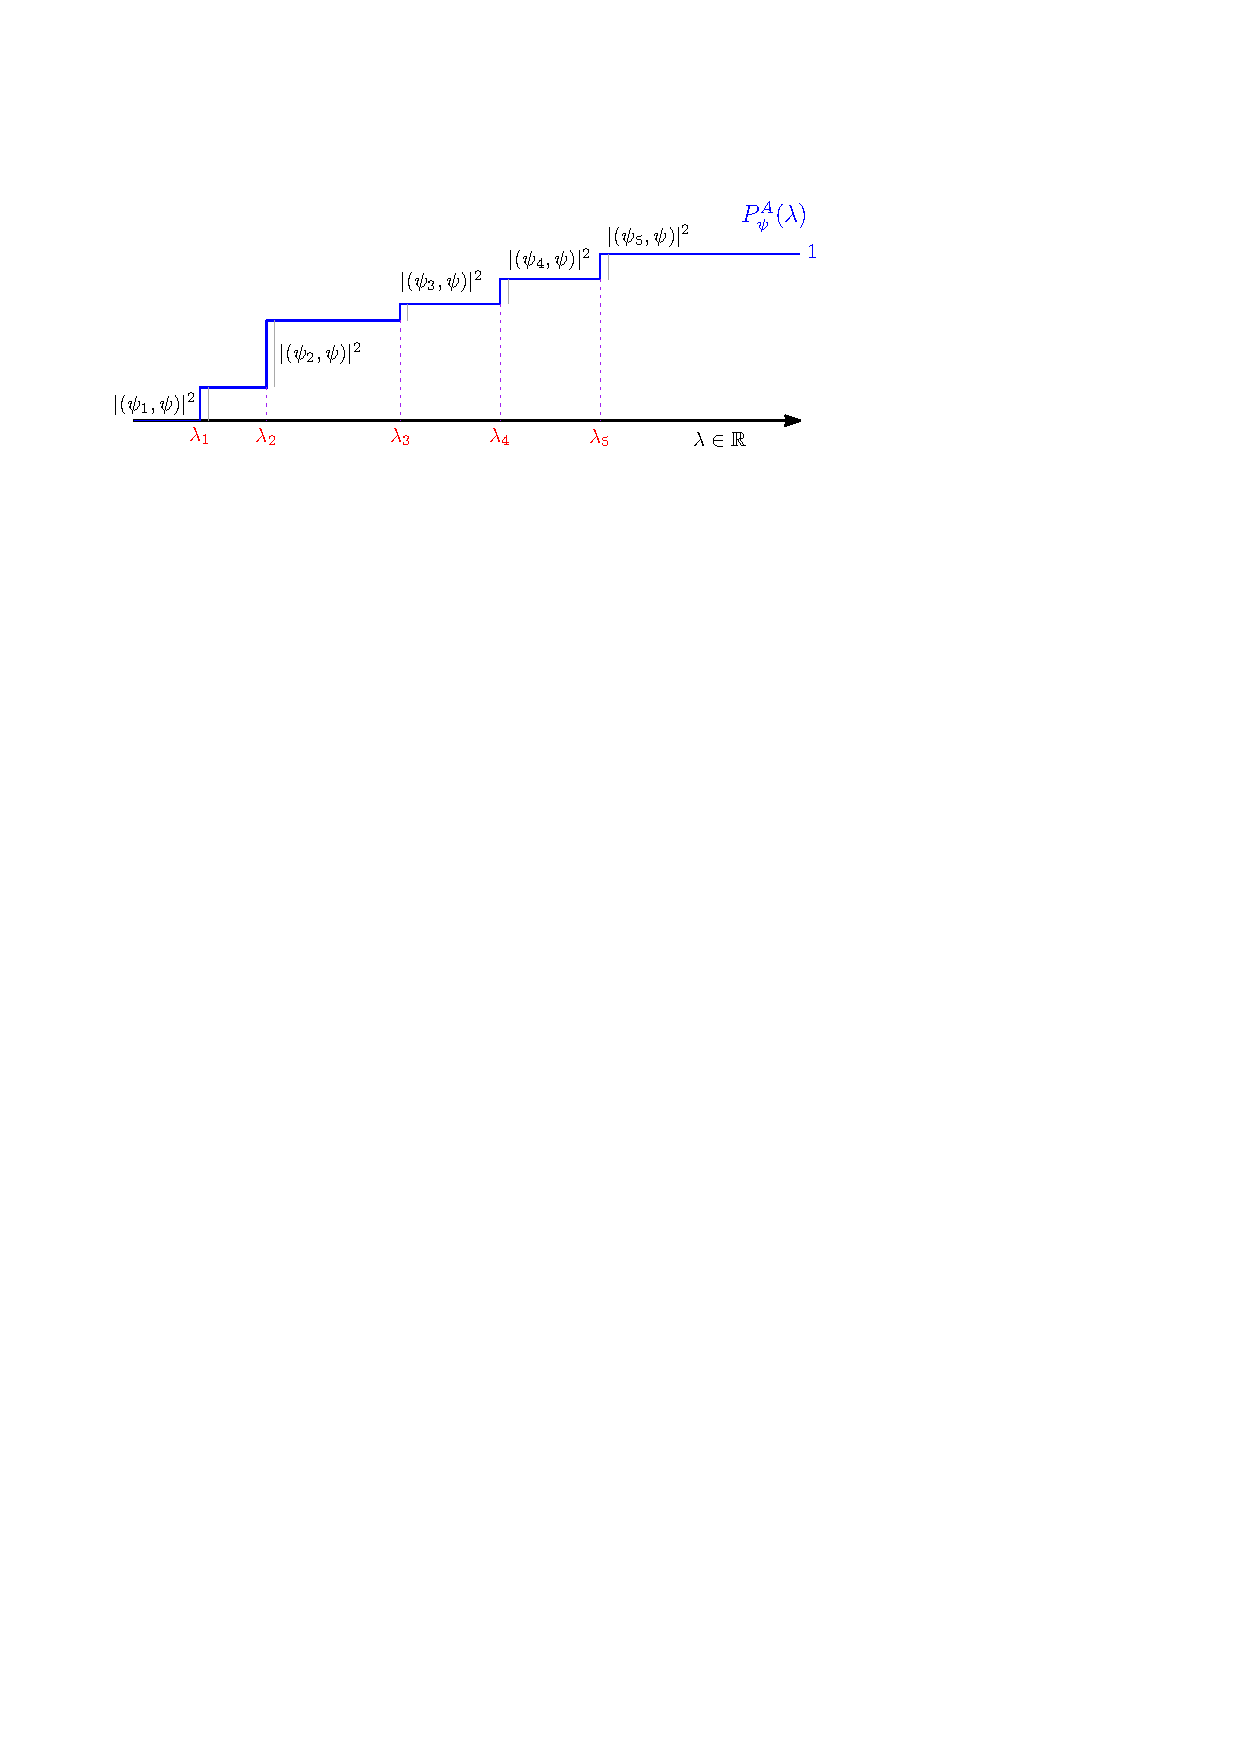
\includegraphics{Immagini/Heaviside.pdf}
    \caption{Andamento di $P_\psi^A(\lambda)$}
    \label{fig:Pautov}
\end{figure}
Supponiamo di porre sulla retta reale gli autovalori, in ordine crescente. In particolare, vi sarà un autovalore minimo $\lambda_1$, prima del quale la $P_\psi^A\left(\lambda\right)$ è nulla. Quando incontra il primo autovalore vi è un \q{gradino} (dato dalla Heaviside), e allo stesso modo per i successivi autovalori, con \q{il salto} tra ciascuno che è dato dal peso $\left|\psi_n,\ \psi\right|^2$, come illustrato in figura \ref{fig:Pautov}.\\
Alla fine (dopo tutti gli autovalori), giungerà ovviamente a $1$, essendo normalizzata la $\psi$ normalizzata: $\norm{\psi}=1$. Perciò:
\[
\sum_{n}\left|(\psi_n,\ \psi\right)|^2=1
\]
In particolare:
\[
P_\psi^A\left(\lambda\right)=\text{ probabilità in una misura di $A$ nello stato $\psi$  di trovare un valore }\leq \lambda 
\]
Perciò costruendo l'operatore $P^A$ grazie alla decomposizione spettrale possiamo ricreare la struttura probabilistica (e in particolare ottenere la \q{probabilità cumulativa} $P^A_\psi$).\\
Elenchiamo ora alcune \textbf{proprietà}\marginpar{Proprietà di $P^A(\lambda)$} degli operatori $\left\{P^A\left(\lambda\right),\ \lambda\in\mathbb{R}\right\}$ dati da $P^A(\lambda) = \sum_n H(\lambda-\lambda_n)P_n$
(siamo sempre nel caso di $\dim{\mathcal{H}}<\infty$). L'idea è di richiedere le stesse proprietà anche nel caso infinito-dimensionale, in modo da svincolarsi dalle equazioni agli autovalori e poter generalizzare.
\begin{enumerate}
    \item $P^A(\lambda)$ è un \textbf{proiettore}\marginpar{$P^A(\lambda)$ è un proiettore}. Infatti è autoaggiunto:
    \[
	\left(\sum_{n}{H\left(\lambda-\lambda_n\right)P_n}\right)^\dag=\sum_{n}{H\left(\lambda-\lambda_n\right)^\ast\ P_n^\dag}=\sum_{n}{H\left(\lambda-\lambda_n\right)P_n}
	\]
	Dove si è usato il fatto che $H$ è reale (quindi pari al suo coniugato), e $P_n$ è autoaggiunto.\\
	Vale anche la seconda condizione per i proiettori, ossia che $P^A(\lambda)^2 = P^A(\lambda)$:
	\begin{equation}
	P^A\left(\lambda\right)^2
	=\left(\sum_{n}{H\left(\lambda-\lambda_n\right)P_n}\right)\left(\sum_{m}{H\left(\lambda-\lambda_m\right)P_m}\right)
	\label{eqn:PAquadro}
	\end{equation}
	Dove si ha che:
	\begin{align*}
	P_nP_m\psi&\underset{(a)}{=}P_n\left(\psi_m,\psi\right)\psi_m \underset{(b)}{=}\left(\psi_m,\psi\right)\left(\psi_n,\psi_m\right)\psi_n \underset{(c)}{=}\\
	&= \delta_{nm}(\psi_m, \psi) \psi_n = 
	\delta_{nm}\underbrace{\braket{\psi_m | \psi}\ket{\psi_n}}_{P_n\psi}  \underset{(d)}{=} 
	P_n\psi\,\delta_{nm}
	\end{align*}
	%[TO DO] \delta_{mn} è una delta di Kronecker, non di Dirac!
	In (a) si applica $P_m$ a $\psi$, che genera $\ket{\psi_m}\braket{\psi_m|\psi}$, mentre in (b) si applica $P_n$ al $\ket{\psi_m}$ appena generato, che porta a $\braket{\psi_n, \psi_m}\ket{\psi_n} \braket{\psi_m|\psi}$. Ma per un operatore simmetrico come $A$ (che è autoaggiunto) possiamo scegliere una base ortonormale di autovettori $\psi_n$, per cui in (c) $\braket{\psi_n|\psi_m} = \delta_{mn}$ (il prodotto scalare restituisce $1$ per la normalizzazione solo quando un vettore è moltiplicato per se stesso, e altrimenti $0$ perché gli autovettori sono ortogonali tra loro). Infine in (d) usiamo la $\delta$ per identificare $n=m$, e riconoscere in $\braket{\psi_m | \psi}\ket{\psi_n}$ il proiettore $P_n$ applicato a $\psi$.\\
	Se consideriamo solo l'operatore \q{puro} avremo perciò $P_n P_m = \hlc{Yellow}{P_n \delta_{nm}}$\\
	Sostituendo questo risultato in (\ref{eqn:PAquadro}):
	\begin{align*}
	P^A(\lambda)^2 &= \sum_{n,m} H(\lambda -\lambda_n)H(\lambda-\lambda_m) \hlc{Yellow}{P_n P_m} = \\
	&= \sum_{n,m}{H\left(\lambda-\lambda_n\right)H\left(\lambda-\lambda_m\right)P_n\delta_{nm}}= \\
	&\underset{(a)}{=} \sum_{n}{H\left(\lambda-\lambda_n\right)H\left(\lambda-\lambda_n\right)P_n}\\
	&\underset{(b)}{=}\sum_{n}{H\left(\lambda-\lambda_n\right)P_n}=P^A\left(\lambda\right)
	\end{align*}
	In (a) abbiamo usato la $\delta$ per identificare $n=m$ e collassare la doppia sommatoria a un'unica variabile.\\
	In (b), invece, si è usato il fatto che la Heaviside assume come valori solo $0$ e $1$, e in particolare è una funzione caratteristica, e il suo quadrato è ovviamente se stessa - in effetti l'avevamo vista come analogo nelle funzioni dei proiettori.
	\item $
	\displaystyle 
	\lim_{\lambda\rightarrow-\infty}{P^A\left(\lambda\right)=0};\quad 
	\lim_{\lambda\rightarrow+\infty}{P^A\left(\lambda\right)}=\sum_{n} P_n=\sum_{n}\left|\psi_n\right\rangle\left\langle\psi_n\right|=\bb{I}
	$\\
	Seguendo\marginpar{Comportamento asintotico di $P^A(\lambda)$} un po' il discorso già fatto per $P_\psi^A(\lambda)$, per $\lambda\to-\infty$ non vi sarà alcun autovalore $\lambda_n \leq \lambda$, e perciò l'operatore darà $0$ (nella definizione, l'Heaviside è costantemente $0$ per $\lambda\to -\infty$). All'estremo opposto, invece, avremo che l'operatore è semplicemente la somma di tutti i proiettori $P_n$ - e la somma di tutte le proiezioni (vettoriali) di un vettore su una base ON è il vettore stesso - da cui l'operatore agisce come l'identità. 
	\item 
	$\displaystyle P^A\left(\lambda\right)P^A\left(\lambda '\right)=P^A\left(\lambda '\right)P^A\left(\lambda\right)=P^A\left(\min{\left\{\lambda,\ \lambda '\right\}}\right) $\\
	Per comprenderlo\marginpar{Composizione di $P^A(\lambda)$} applichiamo la definizione, e concentriamoci sulle Heaviside. In particolare, esaminiamo la seguente espressione nella variabile $\lambda''$:
	\[
	H\left(\lambda-\lambda^{\prime\prime}\right)H(\lambda '-\lambda^{\prime\prime})
	\]
	Il primo termine è $1$ per $\lambda^{\prime\prime}<\lambda$, e il secondo è $1$ solamente se $\lambda^{\prime\prime}<\lambda'$.\\
	Perciò il valore sarà $1$ nell'intersezione tra i due insiemi, che è data da $\lambda^{\prime\prime}<\min{\left\{\lambda,\ \lambda'\right\}}$, e la funzione si può riscrivere come:
	\[
	H\left(\min{\left\{\lambda,\ \lambda '\right\}}-\lambda^{\prime\prime}\right)
	\]
	\item $\displaystyle \lim_{\lambda\rightarrow\lambda_0^+}{P^A\left(\lambda\right)}=P^A(\lambda_0) $\\
	Poiché la Heaviside\marginpar{$P^A(\lambda)$ sono continui a destra} è $1$ in $0$ (è continua da destra, ma non da sinistra), perciò il \q{valore da sopra} è lo stesso della funzione in quel punto. Più precisamente:
	\[
	\lim_{x\rightarrow 0^+}{H \left(x\right)}=1; \quad 
	\lim_{x\rightarrow 0^-}{H\left(x\right)}=0
	\]
\end{enumerate}
\begin{dfn}
Una famiglia di proiettori\marginpar{Famiglia spettrale} $\left\{P\left(\lambda\right),\ \lambda\in\mathbb{R}\right\}$ che soddisfa le proprietà 2-4, è detta \textbf{famiglia spettrale}.
\end{dfn}

\begin{thm}
Esiste una corrispondenza biunivoca\marginpar{Operatore autoaggiunto $\leftrightarrow$ famiglia spettrale} tra operatori autoaggiunti $A=A^\dag$ e famiglie spettrali definita da:
\begin{align}
\nonumber &\left\{P\left(\lambda\right),\lambda\in\mathbb{R}\right\}\rightarrow A\\
D\left(A\right)&= \left\{\phi\in\mathcal{H}\ |\ \int_{\mathbb{R}}{\lambda^2\ d\left(\phi,P\left(\lambda\right)\phi\right)<\infty}\right\} 
\label{eqn:dominiofamigliaspettrale}
\end{align}
Si ha che $D(A)$ è denso, quindi per definire $A$ basta darne gli elementi di matrice:
\[
\left(\phi,A\phi\right)=\int_\bb{R} \lambda\, d\left(\phi,P\left(\lambda\right)\phi\right)
\]
Più in generale, se $f$ è una funzione misurabile su $\bb{R}$, esiste un operatore $f\left(A\right)$ con dominio $D(f(A))$ denso in $\hs$, dato da:
\[
D\left(f\left(A\right)\right)= \left\{\phi\in\mathcal{H}\ |\ \int\left|f\left(x\right)\right|^2d\left(\phi,P\left(\lambda\right)\phi\right)<\infty\right\}
\]
L'operatore $f(A)$ è quindi definito completamente dai suoi elementi di matrice:
\[
\left(\phi,f\left(A\right)\phi\right)=\int f\left(\lambda\right) d(\phi , P\left(\lambda\right)\phi )
\]
(Qui negli elementi di matrice stiamo usando tutti vettori nel dominio denso dell'operatore, poiché abbiamo visto che è possibile utilizzare l'\textbf{identità di polarizzazione} per riscrivere il tutto in termini di valori medi)
\end{thm}
\textbf{Dim.} (molto tecnica e lunga, omessa)\\
In particolare, per la speciale funzione $H(\lambda-A)$ si ha:
\[
H(\lambda-A) = P(\lambda)
\]
(per chiarire, prova a pensare tutto ciò in termini di spazi finito-dimensionali).\\
Con questa strategia non abbiamo usato autovettori/autovalori, e perciò tramite questa è possibile estendere quanto detto nel caso finito-dimensionale all'infinito-dimensionale.

\textbf{Esempio}\index{Famiglia spettrale!operatore posizione $X$} \marginpar{Esempio (1) di famiglia spettrale: operatore posizione}
In $\hs =L^2(\bb{R}, dx)$, consideriamo la \textbf{famiglia spettrale}:
\begin{equation}
\left(P\left(\lambda\right)\psi\right)\left(x\right)=H\left(\lambda-x\right)\psi \left(x\right)
\label{eqn:famiglia_spettrale_x}
\end{equation}
Verifichiamo che soddisfa tutte le proprietà:
\begin{enumerate}
    \item $H$ reale e $H^2=H$, quindi è un proiettore.
    \item 
    $\displaystyle \lim_{\lambda\rightarrow-\infty}{H\left(\lambda-x\right)\psi\left(x\right)=0};
    \quad
	\lim_{\lambda\rightarrow+\infty}{H\left(\lambda-x\right)\psi(x)}=\psi
	\left(x\right)\>\forall \psi \in \hs $
    \item 
    $\displaystyle H\left(\lambda-x\right)H\left(\lambda '-x\right)=H\left(\min{\left\{\lambda,\ \lambda '\right\}}-x\right)$
    \item 
    $\displaystyle \lim_{\lambda\rightarrow\lambda_0^+}{H\left(\lambda-x\right)}=H\left(\lambda_0-x\right)$
\end{enumerate}
Di quale operatore autoaggiunto è la famiglia spettrale? Calcoliamone il dominio:
\begin{align*}
D\left(A\right)&= \left\{\phi\in L^2\left(\mathbb{R}\right)\ |\ \int_\bb{R}\lambda^2\, d\left(\phi,P\left(\lambda\right)\phi\right)<\infty\right\}\\
\left(\phi,P\left(\lambda\right)\phi\right)&=\int_\bb{R} dx\, \phi^\ast\left(\lambda\right)H\left(\lambda-x\right)\phi \left(x\right)\\
d\left(\phi,P\left(\lambda\right)\phi\right)&=\left(\int_\bb{R} dx\,\phi^\ast\left(x\right)\delta\left(\lambda-x\right)\phi\left(x\right)\right)d\lambda =\phi^\ast\left(\lambda\right)\phi \left(\lambda\right)d\lambda 
\end{align*}
E quindi:
\begin{align*}
D\left(A\right)&= \left\{\phi\in L^2\left(\mathbb{R},dx\right)\ \ |\ \ \int\lambda^2\phi^\ast\left(\lambda\right)\phi\left(\lambda\right)\,d\lambda<\infty\right\}= \left\{\left|\left|x\phi\right|\right|^2<\infty\right\}
\end{align*}
E gli elementi di matrice sono dati da:
\begin{align*}
    \left(\phi,A\phi\right)=\int \lambda\, d\left(\phi,P\left(\lambda\right)\phi\right)= \int \lambda\,\phi^\ast\left(\lambda\right)\phi \left(\lambda\right)d\lambda =\int x\,\phi^\ast\left(x\right)\phi \left(x\right)dx
\end{align*}
Riconosciamo l'azione dell'operatore \textbf{posizione}:
\begin{align*}
    X\phi \left(x\right)&=x\,\phi \left(x\right)\\
    D\left(X\right)&=\left\{\phi\in L^2\ |\ \left|\left|x\phi\right|\right|^2<\infty\right\}
\end{align*}
Quindi $A=X$, e $dP_\phi^X(\lambda) = |\phi(\lambda)|^2 d\lambda$.\\
Se $\phi$  non è normalizzato, perché sia \[ \int_{\mathbb{R}}{dP_\phi^X\left(\lambda\right)}=1 \]
Bisogna scrivere:
\[
dP_\phi^X\left(\lambda\right)=\hlc{SkyBlue}{\frac{\left|\phi\left(\lambda\right)\right|^2}{\left|\left|\phi\right|\right|^2}}d\lambda 
\]
La grandezza evidenziata in azzurro è la \textbf{densità di probabilità}\marginpar{Densità di probabilità} che misurando $X$ nello stato $\phi$ si ottenga $\lambda$. In fisica si denota con:
\[
w_\phi^X\left(\lambda\right)=\frac{dP_\phi^X\left(\lambda\right)}{d\lambda}=\frac{\left|\phi\left(\lambda\right)\right|^2}{\left|\left|\phi\right|\right|^2}
\]
Il valor medio è quindi:
\[
\left\langle X\right\rangle_\phi=\int \lambda  dP_\phi^X\left(\lambda\right)=\int \lambda  w_\phi^X\left(\lambda\right) d\lambda 
\]
Riepilogando: \marginpar{Riepilogo delle \textbf{proprietà} delle \textbf{osservabili}}
\begin{enumerate}
    \item Le osservabili sono \textbf{operatori} $A$ e dalla indipendenza del rappresentativo del raggio vettore nel calcolo dei valor medi $\langle A\rangle_\psi$ si ha che $A$ sono \textbf{lineari} (e richiediamo abbiano un dominio denso in $\hs$, ossia il più largo possibile).
    \item Vogliamo poi che $\langle A \rangle_\psi \in \bb{R}$, da cui $A$ deve essere \textbf{simmetrico}.
    \item La richiesta che esista $f\left(A\right)$ implica che $A$ è \textbf{autoaggiunto}.  Ciò consente anche di costruire una interpretazione probabilistica, potendo definire la funzione $P_\psi^A\left(\lambda\right)$
\end{enumerate}
Enunciamo questi risultati, che abbiamo costruito nei paragrafi precedenti e che sono estensivamente corroborati dall'evidenza, come \textbf{assiomi} del formalismo quantistico.
\begin{axi}
Le \textbf{osservabili}\marginpar{Assioma delle osservabili}\index{Assioma!delle osservabili} di un sistema quantistico, i cui \textbf{stati puri} sono descritti dai \textbf{raggi vettori} di $\hs$, sono descritti da \textbf{operatori autoaggiunti} $A=A^\dag$ in $\hs$.
\end{axi}

\begin{axi}
La \textbf{probabilità}\marginpar{Assioma della probabilità}\index{Assioma!della probabilità} che il risultato di una misura di $A$ nello stato $\psi$ (ricavata ripetendo tante volte la misura sperimentale nelle stesse condizioni) sia in $]-\infty , \lambda]$ è data da:
\[
P_\psi^A\left(\lambda\right)=\frac{(\psi,\ P^A\left(\lambda\right)\psi)}{\norm{\psi}^2}
\]
Dove $P^A\left(\lambda\right)$ è la \textbf{famiglia spettrale} di $A$ e $\forall \psi \in D\left(A\right)$:
\[
\langle A \rangle_\psi = \frac{(\psi, A\psi)}{\norm{\psi}^2}
\]
\end{axi}

\subsection{Osservazioni sulle proprietà matematiche delle osservabili}
\begin{enumerate}
    \item La condizione di autoaggiuntezza è delicata: 
	Ad esempio, se $A$ e $B$ sono autoaggiunti \textbf{limitati}, $A+B$ lo è, ma $AB$ no. Infatti $\left(AB\right)^\dag=B^\dag A^\dag=BA\neq AB$.\\
	Perciò gli operatori autoaggiunti non formano un'algebra sui reali.\\
	Possiamo costruire un'algebra degli operatori autoaggiunti su $\bb{C}$, e in effetti $\frac{\left(AB-BA\right)}{i}$ è autoaggiunto.
	\item Se invece $A$ e $B$ sono autoaggiunti, ma \textbf{illimitati} in $D\left(A\right)$ e $D(B)$ densi in $\hs$. Allora $(A+B)$ è ben definito in $D\left(A\right)\cap D\left(B\right)$ ma $A+B$ in generale non è autoaggiunto in $D\left(A\right)\cap D\left(B\right)$ che potrebbe addirittura non essere denso.\\
	Questo problema appare in fisica ad esempio per l'osservabile energia:
	\[
	H=\frac{{\vec{p}}^{\,2}}{2m}+V(\vec{x})
	\]
	Con $A=\frac{{\vec{p}}^2}{2m}, B=V(\vec{x})$\\
	Fortunatamente, molti casi importanti sono coperti dal seguente risultato:
	\begin{thm}
	Se $V$ è limitato in $\mathbb{R}^n$, oppure se $n=3$ e $V$ è Coulombiano (es. potenziale elettrostatico), allora $H$ è autoaggiunto nel dominio di $A$ definito da:
	    \[
	    D\left(\vec{p}^{\>2}\right)=\left\{\varphi\in L^2\left(R^n,\ d^nx\right)\middle|\ {\vec{p}}^{\>2}\widetilde{\varphi}\left(\vec{p}\,\right)\in L^2\left(R^n, d^np\right)\right\}
	    \]
	\end{thm}
	\item \textbf{Attenzione}: Conoscere $\sigma(A)$ e $\sigma(B)$ non porta alla conoscenza di $\sigma(A+B)$.\\
	Per esempio, $A=\frac{p^2}{2m}, B=V\left(x\right)$, con $\sigma \left(A\right)= \mathbb{R}_+, \sigma \left(V\left(x\right)\right)=\op{cod} V(x)$ sono entrambi operatori a spettro continuo. Tuttavia la loro somma contiene uno spettro discreto: sono per esempio i livelli energetici di una buca infinita.\\
	(In \MC, d'altro canto, conoscere $\sigma(A)$ e $\sigma(B)$ porta subito alla conoscenza di $\sigma(A+B)$.)\\
\end{enumerate}
\end{document}